\todo{Auswertungsreihenfolge (applikative, normale)}
\todo{Racket: Wichtige Funktionen (filter, map, foldl, etc.)}
\todo{Java: JUnit}
\todo{Java: Streams}
\todo{Java: Lambdas}



\chapter{HtDP-TL}
    Die HtDP-TL (How to Design Programs-Teaching Language) ist ein Teil der Sprache Racket, welche einen Dialekt von, welches eine implementierung von Lisp (List Processing) darstellt. Die Syntax der HtDP-TL ist äquivalent zu der Syntax von Racket, da HtDP-TL ausschließlich den Funktionsumfang von Racket einschränkt (das heißt es stehen weniger Funktionen zur Verfügung). Im folgenden werden Racket und HtDP-TL äquivalent verwendet, wobei ausschließlich HtDP-TL gemeint ist.

    \section{Syntax}
        Da Racket eine vollfunktionale Sprache ist, existieren keine Variablen, sondern der gesamte Quellcode besteht nur aus Funktionsaufrufen.

        \subsection{Funktionsaufrufe}
            Eine Funktion wird in einem Listenähnlichen konstrukt aufgerufen, wobei der Name der aufzurufenden Funktion am Beginn der Liste steht. Alle Parameter folgen durch ein Leerzeichen getrennt. Der Funktionsaufruf wird mit einer schließenden Klammer abgeschlossen: \texttt{(<Funktionsname> <Parameter 1> <Parameter 2> ... <Parameter n>)}

            \textbf{Fun Fact:} Es ist irrelevant, ob runde, eckige oder geschweifte Klammern verwendet werden. Eine Variation der Klammern ist nur gut für die Lesbarkeit.

            \paragraph{Beispiel}
                \texttt{'+'} stellt die Funktion zum Addieren von beliebig vielen Zahlen dar. Möchte man nun die Zahlen \texttt{24}, \texttt{7} und \texttt{11} addieren, so wird dies wie folgt geschrieben: \texttt{(+ 24 7 11)}



    \subsection{Primitive Datentypen}
        \subsubsection{Beschreibung}
            \begin{description}
                \item[String] Stellt eine folge von Zeichen dar.
                \item[Boolean] Stellt einen Wahrheitswert (Wahr/Falsch) dar.
                \item[Symbol] Stellt ein sogenanntes Symbol dar. Ein Symbol ist prinzipiell ein String, welcher keine Leerzeichen und Klammer (mit Ausnahme von spitzen Klammer) enthalten kann und dynamisch in jeden anderen Typ umgewandelt wird. Konkret bedeuted dies, ein Symbol mit dem Inhalt der syntaktisch korrekt zu einem anderen Datentyp passt (beispielsweise eine Zahl) ist gleichzeitig dieser Datentyp.
                \item[Number] Stellt eine Zahl dar. Außerdem können alle Zahlen sowohl in Binär, Oktal, Dezimal und Hexadezimal eingelesen werden.
                    \begin{description}
                        \item[Integers] Stellen ganze Zahlen dar.
                        \item[Floating Point Numbers] Stellen Fließkommazahlen dar. Diese können, aufgrund der internen Darstellung, Darstellungsfehler enthalten.
                        \item[Factions] Stellen Brüche dar. Racket beherrscht bruchrechnung, das heißt die Berechnung mit Brüchen ist relativ exakt.
                        \item[Complex Numbers] Stellen komplexe Zahlen mit Real- und Imaginäranteil dar.
                    \end{description}
            \end{description}


        \subsubsection{Format}
            \begin{description}
                \item[String] Wird in doppelte Anführungszeich eingefasst, wobei doppelte Anführungszeichen in dem String mit einem Backslash (\texttt{\textbackslash}) maskiert (escaped) werden müssen (d.h. dem Zeichen wird ein Backslash voran gestellt). Soll ein Backslash in dem String enthalten sein, so muss dieses ebenfalls escaped werden (d.h. es müssen zwei Backslashes geschrieben werden). \\ Beispiel: \verb$"Hello, World!"$, \verb$"\"\\"$
                \item[Boolean] Ein Boolean hat nur zwei mögliche Werte, welche allerdings unterschiedlich dargestellt werden können: $ \texttt{true} \iff \texttt{\#t} $, $ \texttt{false} \iff \texttt{\#f} $
                \item[Symbol] Ein Symbol wird eingeleitet durch ein einfaches Anführungszeichen (\verb$'$), gefolgt von seinem Inhalt. Das Symbol wird mit dem ersten Zeichen abgeschlossen, welches ein Symbol nicht enthalten kann (beispielsweise ein Leerzeichen). Da Symbole dynamisch in alle Typen umgewandelt werden, gilt beispielsweise $ \texttt{'123} \iff \texttt{123} $
                und \verb$'"HelloWorld"$ $ \iff $ \verb$HelloWorld$. Falls symbole einen String darstellen (das heißt der Inhalt ist in doppelten Anführungszeichen geschrieben), kann ein Symbol alle Zeichen beinhalten (Beispiel: \verb$'"Hello, World!"$ $ \iff $ \verb$"Hello, World!"$).
                \item[Number]
                    \begin{description}
                        \item[Integers] Die darzustellende Zahl wird einfach in den Quellcode geschrieben. Vor der Zahl kann ein Minus als Vorzeichen stehen. \\ Beispiel: \texttt{42}
                        \item[Floating Point Numbers] Die Nachkommastellen werden durch einen Punkt von dem ganzzahligen Teil der Zahl getrennt. Vor der Zahl kann ein Minus als Vorzeichen stehen. \\ Beispiel: \texttt{123.45} \\ Sind keine Nachkommastellen vorhanden, wird der Punkt weg gelassen und die Zahl stellt eine Ganzzahl dar.
                        \item[Factions] Der ganzzahlige Zähler wird mit einem Schrägstrich von dem ganzzahligen nenner getrennt. Dabei darf zwischen dem Schrägstrich und den Zahlen kein Leerzeichen stehen. Vor der Zahl kann ein Minus als Vorzeichen stehen. \\ Beispiel: \texttt{12/34}
                        \item[Complex Numbers] Komplexe Zahlen werden dargestellt durch den Realanteil, gefolgt von dem Imaginäranteil und einem \texttt{i}. Dabei muss zwischen dem Real- und Imaginäranteil ein Plus oder ein Minus stehen. Ebenfalls kann der Realanteil positiv oder negativ sein. Zwischen allen Zeichen darf kein Leerzeichen stehen. \\ Beispiel: \texttt{12+34i}, \texttt{-12-34i}
                    \end{description}
            \end{description}



    \subsection{Komplexe Datentypen}
        \subsubsection{Listen}
            Listen sind in Racket als sogenannte gelinkte Liste implementiert, das heißt jeder Listeneintrag hält das ihm zugehörige Element und einen Zeiger auf den nächsten Listeneintrag, welcher wiederrum einen Zeiger auf das nächste Listenelement hält und so weiter. Das letzte Listenelement hält einen Zeiger auf die leere Liste, um die gesamte Liste abzuschließen. Das Bild \ref{f:linked_list} visualisiert dieses Verhalten anhand eines Beispiels.

            \begin{figure}[ht]
                \label{f:linked_list}
                \centering
                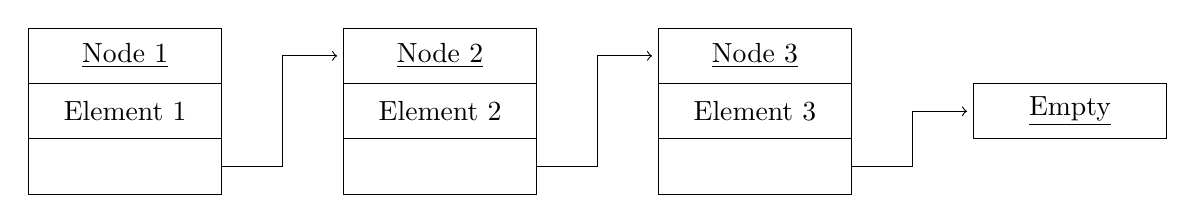
\begin{tikzpicture}[main node/.style = {draw, rectangle, minimum size = 20pt, minimum width = 70pt}]
                    \node at (0, 0) [main node] (node1) {\underline{Node 1}};
                    \node at (0, -20pt) [main node] (element1) {Element 1};
                    \node at (0, -40pt) [main node] (pointer1) {};
                    \node at (4, 0)[main node] (node2) {\underline{Node 2}};
                    \node at (4, -20pt) [main node] (element2) {Element 2};
                    \node at (4, -40pt) [main node] (pointer2) {};
                    \node at (8, 0)[main node] (node3) {\underline{Node 3}};
                    \node at (8, -20pt) [main node] (element3) {Element 3};
                    \node at (8, -40pt) [main node] (pointer3) {};
                    \node at (12, -20pt)[main node] (node4) {\underline{Empty}};
                    \coordinate (mid12) at (2, -20pt);
                    \coordinate (mid23) at (6, -20pt);
                    \coordinate (mid34) at (10, -20pt);

                    \draw (pointer1) -| (mid12);
                    \draw [->, shorten >= 2pt] (mid12) |- (node2);
                    \draw (pointer2) -| (mid23);
                    \draw [->, shorten >= 2pt] (mid23) |- (node3);
                    \draw (pointer3) -| (mid34);
                    \draw [->, shorten >= 2pt] (mid34) |- (node4);
                \end{tikzpicture}
                \caption{Gelinkte Liste}
            \end{figure}

            Die folgenden Abschnitte fassen kurz die primitiven Operationen auf Listen in Racket zusammen.

            \paragraph{Die leere Liste}
                Die leere Liste ist als \texttt{empty} vorhanden.

            \paragraph{Hinzufügen eines Elementes an eine Liste}
                \begin{description}
                    \item[Abstraktes Konstrukt] \texttt{(cons <element> <list>)}
                    \item[Vertrag] \texttt{cons :: any list $ \rightarrow $ list}
                    \item[Beispiel] \texttt{(cons 'a (cons 'b lst))}
                    \item[Warnung] Dies fügt das Element nicht wirklich zu der Liste hinzu, sondern erstellt eine neue Liste!
                \end{description}

            \paragraph{Erstellen einer Liste mit bekannten Elementen}
                Eine neue Liste kann mittels \texttt{cons} erstellt werden. Beispiel: \texttt{(cons 'a (cons 'b empty))}

                Da dies relativ viel Schreibarbeit ist, kann auch folgendes Konstrukt mit dem gleichen Effekt verwendet werden:
                \begin{description}
                    \item[Abstraktes Konstrukt] \texttt{(list [element]...)}
                    \item[Vertrag] \texttt{list :: any...}
                \end{description}

                Alternativ ist folgendes Konstrukt verfügbar:
                \begin{description}
                    \item[Abstraktes Konstrukt] \texttt{'([element]...)}
                    \item[Beispiel] \verb$'(a b "Hello, World!")$ $ \rightarrow $ \verb$(list 'a 'b '"Hello, World!")$
                    \item[Warnung] Jedes Element der Liste wird zu einem Symbol, bzw. zu dem jeweiligen Typen!
                \end{description}

            \paragraph{Prüfen, ob X eine Liste ist}
                \begin{description}
                    \item[Abstraktes Konstrukt] \texttt{(list? <arg>)}
                    \item[Vetrag] \texttt{list? :: any $ \rightarrow $ boolean}
                \end{description}

            \paragraph{Prüfen, ob X leer ist}
                \begin{description}
                    \item[Abstraktes Konstrukt] \texttt{(empty? <arg>)}
                    \item[Vertrag] \texttt{empty? :: any $ \rightarrow $ boolean}
                \end{description}



    \subsection{Kontrollstrukturen}
        \subsubsection{Notation}
            Für jede Kontrollstruktur wird der Name, das Abstrakte Konstrukt, der Vertrag der Kontrollstruktur, eine Beschreibung und ein Beispiel angegeben.


        \subsubsection{If-Statement}
            \label{racket:if}
            \begin{description}
                \item[Name] If-Statement
                \item[Abstraktes Konstrukt] \texttt{(if <condition> <then> <else>)}
                \item[Vertrag] \texttt{if :: boolean any any $ \rightarrow $ any}
                \item[Beschreibung] Liefert \texttt{<condition>} \texttt{true}, so wird das Ergebnis von \texttt{<then>} zurück gegeben. Liefert \texttt{<condition>} \texttt{false}, so wird das Ergebnis von \texttt{<else>} zurück gegeben.
                \item[Beispiel] \texttt{(if (> x y) x y)} Dies stellt eine implementierung der Max-Funktion dar, welche die größere Zahl von zweien liefert.
            \end{description}


        \subsubsection{Cond-Statement}
            \label{racket:cond}
            \begin{description}
                \item[Name] Cond-Statement
                \item[Abstraktes Konstrukt] \texttt{(cond (<condition> <statement>)... [(else <else-statement>)])}
                \item[Vertrag] \texttt{cond :: (boolean any)... (else any)? $ \rightarrow $ any}
                \item[Beschreibung] Liefert \texttt{<condition>} eines condition-statement-tupels \texttt{true}, so wird das Ergebnis des dazugehörigen \texttt{<statement>} zurück geliefert. Die Paare werden dabei von links nach rechts abgefragt, wobei das Ergebnis des erste Paares dessen \texttt{<condition>} \texttt{true} liefert, zurück gegeben wird. Existiert kein solches Paar, so wird das Ergebnis von \texttt{<else-statement>} zurück gegeben. Da dieses optional ist wird, sollte kein else-statement existieren, ein Fehler ausgelöst.
                \item[Beispiel] \texttt{(cond [(> x 2) 'x\_greater\_2] [(> x 1) 'x\_greater\_1] [else 'x\_smaller\_1])} Dies stellt eine Funktion da, die für x mit \texttt{x > 2} das Symbol \texttt{'x\_greater\_2}, für x mit \texttt{x > 1} das Symbol \texttt{'x\_greater\_1} und ansonsten das Symbol \texttt{'x\_smaller\_1} liefert. Hier ist auch zu sehen, wie die Variation von Klammertypen dazu eingesetzt werden kann, den Code übersichtlicher zu gestalten.
            \end{description}



    \subsection{Überblick über die Funktionen}
        \begin{sidewaystable}
            \centering
            \begin{tabular}{p{5cm} | p{7cm} | p{9cm}}
                Name & Vertrag & Beschreibung \\
                \hline
                Addition & \texttt{+ :: number... $ \rightarrow $ number} & Summiert die gegebenen Parameter auf. \\
                Subtraktion & \texttt{- :: number number $ \rightarrow $ number} & Subtrahiert den zweiten von dem ersten Parameter. \\
                Multiplikation & \texttt{* :: number... $ \rightarrow $ number} & Multipliziert die gegebenen Parameter miteinander. \\
                Quadrat & \texttt{sqr :: number $ \rightarrow $ number} & Errechnet das Quadrat der gegebenen Zahl. \\
                Quadratwurzel & \texttt{sqrt :: number $ \rightarrow $ number} & Errechnet die Quadratwurzel der gegebenen Zahl. \\
                Potenz & \texttt{expt :: number number $ \rightarrow $ number} & Berechnet die erste Zahl hoch den zweiten. \\
                \hline
                Null & \texttt{zero? :: number $ \rightarrow $ boolean} & Prüft, ob die gegebene Zahl gleich Null ist. \\
                Gerade & \texttt{even? :: number $ \rightarrow $ boolean} & Prüft, ob die gegebene Zahl gerade ist. \\
                Ungerade & \texttt{odd? :: number $ \rightarrow $ boolean} & Prüft, ob die gegebene Zahl ungerade ist. \\
                \hline
                Division & \texttt{/ :: number number $ \rightarrow $ number} & Dividiert den ersten durch den zweiten Parameter. \\
                Minimaler Wert & \texttt{min :: number... $ \rightarrow $ number} & Gibt das kleinste Element zurück. \\
                Maximaler Wert & \texttt{max :: number... $ \rightarrow $ number} & Gibt das größte Element zurück. \\
                Absoluter Wert & \texttt{abs :: number $ \rightarrow $ number} & Gibt den absoluten Wert der gegebenen Zahl zurück. \\
                Modulo & \texttt{modulo :: number number $ \rightarrow $ number} & Errechnet den Divisionsrest. \\

                \hline
                Größer & \texttt{> :: number number $ \rightarrow $ boolean} & Prüft, ob die erste Zahl größer als die zweite ist. \\
                Kleiner & \texttt{> :: number number $ \rightarrow $ boolean} & Prüft, ob die erste Zahl kleiner als die zweite ist. \\
                Größer-Gleich & \texttt{> :: number number $ \rightarrow $ boolean} & Prüft, ob die erste Zahl größer-gleich die zweite ist. \\
                Kleiner-Gleich & \texttt{> :: number number $ \rightarrow $ boolean} & Prüft, ob die erste Zahl kleiner-gleich die zweite ist. \\
                Gleichheit & \texttt{equal? :: any any $ \rightarrow $ boolean} & Prüft, ob die gegebenen Parameter gleich sind. \\
                \hline
                Erstes Element & \texttt{first :: (listof X) $ \rightarrow $ X} & Gibt das erste Element der Liste zurück. \\
                Zweites Element & \texttt{second :: (listof X) $ \rightarrow $ X} & Gibt das zweite Element der Liste zurück. \\
                $ {}\vdots{} $ & $ {}\vdots{} $ & $ {}\vdots{} $ \\
                Achtes Element & \texttt{eighth :: (listof X) $ \rightarrow $ X} & Gibt das achte Element der Liste zurück. \\
                Rest der Liste & \texttt{rest :: (listof X) $ \rightarrow $ (listof X)} & Gibt den Rest der Liste zurück. \\
                Länge der Liste & \texttt{length :: (listof X) $ \rightarrow $ number} & Gibt die Länge der Liste zurück. \\
                \hline
                If-Statement & & Siehe \ref{racket:if}. \\
                Cond-Statement & & Siehe \ref{racket:cond}. \\
            \end{tabular}
            \caption{Racket: Funktionsüberblick 1}
        \end{sidewaystable}

        \begin{sidewaystable}
            \centering
            \begin{tabular}{p{5cm} | p{7cm} | p{9cm}}
                Name & Vertrag & Beschreibung \\
                \hline
                Datenmapping & \texttt{map :: (X $ \rightarrow $ Y) (listof X) $ \rightarrow $ (listof Y)} & Führt die übergebene Funktion für jedes Element der Liste aus und erstellt eine neue Liste, welche die zurückgegebenen Werte enthält. \\
                Datenfilterung & \texttt{filter :: (X $ \rightarrow $ boolean) (listof X) $ \rightarrow $ (listof X)} & Erstellt eine neue Liste, welche alle Werte aus der alten Liste enthält, für die das übergebene Prädikat \texttt{true} geliefert hat. \\
                Akkumulation der Daten & \texttt{foldl :: (X Y $ \rightarrow $ Y) Y (listof X) $ \rightarrow $ Y} & Fasst die Daten mit Hilfe der übergebenen Funktion von links zusammen. \\
                Leere Liste & \texttt{empty? :: (listof X) $ \rightarrow $ boolean} & Prüft, ob die Liste leer ist. \\
                \hline
                Definition von Konstanten & \texttt{(define <name> <value>)} & Definiert eine Konstante mit dem gegebenen Namen und dem gegebenen Wert. Dieser kann ein Ausdruck sein. \\
                Definition von Funktionen & \texttt{(define (<name> <arg1> <arg2> ... <argN>) <expr>)} & Definiert eine Funktion mit dem gegebenen Namen und den gegebenen Parametern. In dem Ausdruck \texttt{<expr>} können diese genutzt werden. \\
                \hline
                Konjunktion & \texttt{and :: boolean... $ \rightarrow $ boolean} & Stellt ein logisches UND dar. \\
                Disjunktion & \texttt{or :: boolean... $ \rightarrow $ boolean} & Stellt ein logisches ODER dar. \\
                Negation & \texttt{not :: boolean $ \rightarrow $ boolean} & Stellt ein logisches NICHT dar. \\
                \hline
                Test auf Gleichheit & \texttt{(check-expect <actual: any> <expected: any>)} & Testet, ob \texttt{<actual>} dem Wert \texttt{<expected>} entspricht. \\
                Test auf Ähnlichkeit & \texttt{(check-within <actual: number> <expected: number> <delta: number>)} & Testet, ob \texttt{<actual>} und \texttt{<expected>} sich um maximal \texttt{<delta>} unterscheiden. \\
                \hline
                Feld von Struktur selektieren \texttt{(<struct>-<field> <value>)} & Gibt den Wert des Feldes \texttt{<field>} der Struktur \texttt{<struct>} und dem Wert \texttt{<value>} zurück. \\
                \hline
                Lambda & \texttt{(lambda (<param1> <param2> ... <paramN>) <expr>)} & Erstellt eine anonyme Funktion mit den Parametern \texttt{<param1>}, \texttt{<param2>}, \dots, \texttt{<paramN>}, die den Ausdruck \texttt{<expr>} darstellt. \\
                Lexikalischer Scope & \texttt{(local (<define>...) <expr>)} & Erstellt einen neuen lexikalischen Scope, in dessen Audruck \texttt{<expr>} alle Definition aus dem \texttt{define}-Block verfügbar sind. \\
            \end{tabular}
            \caption{Racket: Funktionsüberblick 2}
        \end{sidewaystable}




\chapter{Java}
    \subsection{Streams und Lambdas}
        Java 8 Streams (\texttt{java.util.stream}) bringen funktionale Programmierung in Java ein. Durch Lambdas wird diese kürzer.

        Die besten Wege, um an einen \texttt{java.util.stream.Stream<T>} zu kommen, sind die folgenden:
        \begin{itemize}
            \item Mittels einer \texttt{Collection} (\texttt{List} oder \texttt{Set}): \texttt{java.util.Collection\#stream()}
            \item Mittels eines Arrays: \texttt{java.util.Arrays\#stream(T[])}
        \end{itemize}



    \subsection{Generics}
        \subsubsection{Merksatz}
            Greift man lesend auf generische Typen zu, so sollte man \texttt{extends} verwenden.

            \noindent Greift man schreibend auf generische Typen zu, so sollte man \texttt{super} verwenden.



    \subsection{JUnit}
        Generell müssen alle Methoden in JUnit-Testklassen \texttt{public} sein mit dem Rückgabetyp \texttt{void}. Alle Annotation müssen an solchen Methoden stehen. Ferner kann jede Methode jeden beliebigen Fehler deklarieren (\texttt{throws}). Es kann Sinnvoll sein, einfach \texttt{Exception} zu werfen.

        \subsubsection{Annotationen}
            \begin{sidewaystable}
                \centering
                \begin{tabular}{l | p{9cm} | p{10cm}}
                    Annotation & Parameter & Beschreibung \\
                    \hline
                    \texttt{@BeforeClass} & - & Die Methode wird vor dem initialisieren der Klasse ausgeführt. Die Methode muss \texttt{static} sein! \\
                    \texttt{@AfterClass} & - & Die Methode wird nach dem Ausführen der gesamten Klasse ausgeführt. Die Methode muss \texttt{static} sein! \\
                    \texttt{@Before} & - & Die Methode wird vor jedem Test ausgeführt. \\
                    \texttt{@After} & - & Die Methode wird nach jedem Test ausgeführt. \\
                    \texttt{@Test} & \texttt{expected: Class<? extends Exception>} - Der erwartete Fehler. & Markiert eine Methode als Test. \\
                    & \texttt{timeout: long} - Eine Zeit, in Millisekunden, nach der der Test abgebrochen werden soll. & \\
                \end{tabular}
                \caption{Java: JUnit: Annotationen}
            \end{sidewaystable}


        \subsubsection{\texttt{Assert}}
            \begin{sidewaystable}
                \centering
                \begin{tabular}{l | p{8cm}}
                    Methode & Beschreibung \\
                    \hline
                    \texttt{void assertTrue(boolean actual)} & Schlägt fehl, wenn \texttt{actual} \texttt{false} ist. \\
                    \texttt{void assertFalse(boolean actual)} & Schlägt fehl, wenn \texttt{actual} \texttt{true} ist. \\
                    \texttt{<T> void assertArrayEquals(T[] expected, T[] actual)} & Schlägt fehl, wenn \texttt{actual} sich von \texttt{expected} unterscheidet. \\
                    \texttt{void assertArrayEquals(double[] expected, double[] actual, double delta)} & Schlägt fehl, wenn \texttt{actual} sich mehr als \texttt{delta} von \texttt{expected} unterscheidet. \\
                    \texttt{<T> void assertEquals(T expected, T actual)} & Schlägt fehl, wenn \texttt{actual} sich von \texttt{expected} unterscheidet. \\
                    \texttt{void assertEquals(double expected, double actual, double delta)} & Schlägt fehl, wenn \texttt{actual} sich mehr als \texttt{delta} von \texttt{expected} unterscheidet. \\
                    \texttt{void fail()} & Lässt den Test fehlschlagen. \\
                \end{tabular}
                \caption{Java: JUnit: \texttt{Assert}}
            \end{sidewaystable}




    \subsection{Überblick über die Standardbibliothek}
        \subsubsection{\texttt{Collection<E>}}
            Alle funktionalen Interfaces sind in \ref{java:funcinterf} zusammengefasst.

            \begin{sidewaystable}
                \centering
                \begin{tabular}{l | p{8cm} | c | c}
                    Methode & Beschreibung & List & Set \\
                    \hline
                    \texttt{add(E element)} & Fügt das gegebene Element hinzu. & \texttimes & \texttimes \\
                    \texttt{addAll(Collection<? extends E> elements)} & Fügt alle gegebenen Elemente hinzu. & \texttimes & \texttimes \\
                    \texttt{clear()} & Leert die Liste/Menge. & \texttimes & \texttimes \\
                    \texttt{boolean contains(Object o)} & Prüft, ob das gegebene Objekt vorhanden ist. & \texttimes & \texttimes \\
                    \texttt{boolean containsAll(Collection<?> c)} & Prüft, ob alle gegebenen Objekte vorhanden sind. & \texttimes & \texttimes \\
                    \texttt{boolean isEmpty()} & Prüft, ob die Liste/Menge leer ist. & \texttimes & \texttimes \\
                    \texttt{remove(Object o)} & Entfernt das gegebene Objekt. & \texttimes & \texttimes \\
                    \texttt{removeAll(Collection<?> c)} & Entfernt alle gegebenen Objekte. & \texttimes & \texttimes \\
                    \texttt{Stream<E> stream()} & Wandelt die Liste/Menge in einen Stream um. & \texttimes & \texttimes \\
                    \texttt{<T> T[] toArray(T[] a)} & Wandelt die Liste/Menge in ein Array des gegebenen Types um. & \texttimes & \texttimes \\
                    \texttt{add(int index, E element)} & Fügt das gegebene Element in die Liste an der gegebenen Position ein. & \texttimes & \\
                    \texttt{addAll(int index, Collection<? extends E> elements)} & Fügt alle gegebenen Elemente in die Liste an der gegebenen Position ein. & \texttimes & \\
                    \texttt{E get(int index)} & Gibt das Element an der gegebenen Position zurück. & \texttimes & \\
                    \texttt{int indexOf(Object o)} & Gibt den Index des ersten Eintrages des gegebenen Objektes zurück. & \texttimes & \\
                    \texttt{int lastIndexOf(Object o)} & Gibt den Index des letzten Eintrages des gegebenen Objektes zurück. & \texttimes & \\
                    \texttt{remove(int index)} & Entfernt das Element an der gegebenen Position. & \texttimes & \\
                    \texttt{set(int index, E element)} & Setzt das Element an der gegebenen Position. & \texttimes & \\
                \end{tabular}
                \caption{Java: Funktionsübersicht: \texttt{Collection<E>}}
            \end{sidewaystable}


        \subsubsection{\texttt{Stream<T>}}
            Alle funktionalen Interfaces sind in \ref{java:funcinterf} zusammengefasst.

            \begin{sidewaystable}
                \centering
                \begin{tabular}{p{8cm} | p{13cm}}
                    Methode & Beschreibung \\
                    \hline
                    \texttt{boolean allMatch(Predicate<? super T> pred)} & Prüft, ob das übergebene Prädikat für alle Elemente \texttt{true} liefert. \\
                    \texttt{boolean anyMatch(Predicate<? super T> pred)} & Prüft, ob das übergebene Prädikat für mindestens ein Elemente \texttt{true} liefert. \\
                    \texttt{boolean noneMatch(Predicate<? super T>)} & Prüft, ob das übergebene Prädikat für kein Element \texttt{true} liegert. \\
                    \texttt{<R, A> R collect(Collector<? super T, A, R>)} & Führt den übergebenen \texttt{Collector} auf der Liste aus. Hierbei wird meist die Klasse \texttt{Collectors} verwendet, welche einige Standard-Collectors zur verfügung stellt. Siehe \ref{java:collectors}. \\
                    \texttt{long count()} & Zählt die im Stream enthaltenen Elemente. \\
                    \texttt{Optional<T> findAny()} & Gibt eines der Elemente zurück. Siehe \ref{java:optional}. \\
                    \texttt{Optional<T> findFirst()} & Gibt das erste Element zurück. Siehe \ref{java:optional}. \\
                    \texttt{void forEach(Consumer<? super T> cons} & Führt den übergebenen \texttt{Consumer} auf jedem Element aus. \\
                    \texttt{Optional<T> max()} & Gibt das größte Element zurück. Siehe \ref{java:optional}. \\
                    \texttt{Optional<T> max(Comparator<? super T>)} & Gibt das größte Element auf Basis des übergebenen \texttt{Comparator}s zurück. Siehe \ref{java:optional}. \\
                    \texttt{Optional<T> min()} & Gibt das kleine Element zurück. Siehe \ref{java:optional}. \\
                    \texttt{Optional<T> min(Comparator<? super T>)} & Gibt das kleinste Element auf Basis des übergebenen \texttt{Comparator}s zurück. Siehe \ref{java:optional}. \\
                    \texttt{<U> reduce(U init, BiFunction<U, ? super T, U> accumulator, BinaryOperator<U> combiner)} & Führt eine reduce-Funktion auf dem Stream aus. Dies entspricht dem \texttt{fold} in Racket, wobei der \texttt{combiner} zwei unabhängige Ergebnisse zusammen führt (Sichwort: parallele Programmierung). \\
                    \hline
                    \texttt{Stream<T> distinct()} & Erstellt einen Stream mit einzigartigen Elementen zurück. \\
                    \texttt{Stream<T> filter(Predicate<? super T> pred)} & Erstellt einen neuen Stream, der alle Elemente enthält, für die das übergebene Prädikat \texttt{true} liefert. \\
                    \texttt{Stream<T> limit(long limit)} & Erstellt einen neuen Stream mit maximal \texttt{limit} Elementen. \\
                    \texttt{<R> Stream<R> map(Function<? super T, ? extends R> mapper)} & Erstellt einen neuen Stream, wobei für jedes Element die übergebene Funktion ausgeführt wird und das Ergebnis in den neuen Stream inkludiert wird. \\
                    \texttt{XXXStream mapToXXX(ToXXXFunction<? super T>) mapper} & Das selbe wir \texttt{map(\dots)}, nur dass hierbei auf einen primitiven Typ (\texttt{XXX}) projeziert wird. \\
                    \texttt{Stream<T> sorted()} & Sortiert den Stream. \\
                    \texttt{Stream<T> sorted(Comparator<? super T> comp)} & Sortiert den Stream auf Basis des übergebenen \texttt{Comparator}s. \\
                \end{tabular}
                \caption{Java: Funktionsübersicht: \texttt{Stream<E>}}
            \end{sidewaystable}


        \subsubsection{\texttt{Collectors}}
            \label{java:collectors}
            \begin{sidewaystable}
                \centering
                \begin{tabular}{p{8cm} | p{13cm}}
                    Methode & Beschreibung \\
                    \hline
                    \texttt{static Collector<CharSequence, ?, String> joining(CharSequence delimiter)} & Erstellt einen \texttt{Collector}, der alle Elemente zu einem String zusammenführt, von \texttt{delimiter} getrennt. \\
                    \texttt{static <T> Collector<T, ?, List<T>> toList()} & Erstellt einen \texttt{Collector}, der alle Elemente in eine Liste einfügt. \\
                    \texttt{static <T> Collector<T, ?, Set<T>> toSet()} & Erstellt einen \texttt{Collector}, der alle Elemente in ein Set einfügt. \\
                \end{tabular}
                \caption{Java: Funktionsübersicht: \texttt{Collectors}}
            \end{sidewaystable}


        \subsubsection{\texttt{Optional<T>}}
            \label{java:optional}
            \begin{sidewaystable}
                \centering
                \begin{tabular}{l | l}
                    Methode & Beschreibung \\
                    \hline
                    \texttt{T get()} & Gibt den Wert zurück oder wirft einen Fehler, falls keiner existiert. \\
                    \texttt{boolean isPresent()} & Prüft, ob ein Wert vorhanden ist. \\
                    \texttt{T orElse(T other)} & Gibt den gespeicherten Wert zurück oder, falls keiner vorhanden ist, den übergebenen. \\
                \end{tabular}
                \caption{Java: Funktionsübersicht: \texttt{Optional<T>}}
            \end{sidewaystable}


        \subsubsection{Funktionale Interfaces}
            \label{java:funcinterf}
            \begin{sidewaystable}
                \centering
                \begin{tabular}{l | l}
                    Interface & Methode \\
                    \hline
                    \texttt{java.util.function.Consumer<T>} & \texttt{void accept(T)} \\
                    \texttt{java.util.function.Function<T, R>} & \texttt{R apply(T)} \\
                    \texttt{java.util.function.Predicate<T>} & \texttt{boolean test(T)} \\
                    \texttt{java.util.function.Supplier<T>} & \texttt{T get()} \\
                    \texttt{java.util.function.UnaryOperator<T, T>} & \texttt{T apply(T)} \\
                    \texttt{java.util.function.BiConsumer<T, U>} & \texttt{void accept(T, U)} \\
                    \texttt{java.util.function.BiFunction<T, R, U>} & \texttt{R apply(T, U)} \\
                    \texttt{java.util.function.BinaryOperator<T>} & \texttt{T apply(T, T)} \\
                    \texttt{java.util.function.BiPredicate<T, U>} & \texttt{boolean test(T, U)} \\
                \end{tabular}
                \caption{Java: Funktionsübersicht: Funktionale Interfaces}
            \end{sidewaystable}
